% Für Bindekorrektur als optionales Argument "BCORfaktormitmaßeinheit", dann
% sieht auch Option "twoside" vernünftig aus
% Näheres zu "scrartcl" bzw. "scrreprt" und "scrbook" siehe KOMA-Skript Doku
\documentclass[12pt,a4paper,titlepage,headinclude]{scrartcl}

%%%%%%%%%%%%%%%%%%%%%%%%%%%%%% Formatierung %%%%%%%%%%%%%%%%%%%%%%%%%%%

%keine Einrückung nach leerzeile
\parindent0pt

% Für Kopf und Fußzeilen, siehe auch KOMA-Skript Doku
\usepackage[komastyle]{scrpage2}
\pagestyle{scrheadings}
\setheadsepline{0.5pt}[\color{black}]
\automark[section]{chapter}

%Zitate und Literaturverzeichnis
\usepackage[backend=bibtex,natbib=true,sorting=nyt,style=numeric-comp]{biblatex}
\usepackage[babel,german=quotes]{csquotes}
\bibliography{literatur}

%Zur vernünftigen Dekodierung
\usepackage[T1]{fontenc} %
\usepackage[utf8]{inputenc} %utfx8
\usepackage[ngerman]{babel} %

%Interaktives Dokument
\usepackage[pdfpagelabels=true]{hyperref}%

%Für wissenschaftliches Zitieren
%\usepackage{natbib}

%Schriftarten
%\usepackage{lmodern} %

%Formatierung für Kof- und Fußzeile. Hier gilt entweder ... oder ...!!

%Für eigenen Zeilenabstand
\usepackage{setspace} %



%Für die Seitenformatierung
\usepackage{lscape} %
\usepackage{multicol} %
\usepackage{wallpaper} %

%Styling Inhaltsverzeichnis
\usepackage{tocloft} %

% Zur Formatierung für Kopf und Fußzeilen. Im Allgemeinen ist scrpage2 besser als fancyhdr
\usepackage{scrpage2}
\pagestyle{scrheadings}
\setheadsepline{0.5pt}[\color{black}]

%Einstellungen für Figuren- und Tabellenbeschriftungen
\setkomafont{captionlabel}{\sffamily\bfseries}
\setcapindent{0em} 


%%%%%%%%%%%%%%%%%%%%%%%%%%%%%% Mathematisches %%%%%%%%%%%%%%%%%%%%%%%%%%%

%Pakete für Mathesymbole
\usepackage{latexsym,exscale,stmaryrd} %
\usepackage{amssymb, amsfonts, amstext} %
\usepackage{amsmath, mathtools, amsthm} %

%Formelnummerierungen
\numberwithin{equation}{section}

% Weitere Symbole
\usepackage[nointegrals]{wasysym} %
\usepackage{eurosym} %
\usepackage{textcomp} %

%\usepackage{ucs} %

%Für vernünftige Einheiten 
\usepackage[separate-uncertainty, exponent-product = \cdot]{siunitx}
%\usepackage[thinspace,thinqspace,amssymb]{SIunits} %
\usepackage{icomma} %
\usepackage{nicefrac}%

%SI-Einheiten
\usepackage{siunitx}

%%%%%%%%%%%%%%%%%%%%%%%%%%%%%% Grafiken & Tabellen %%%%%%%%%%%%%%%%%%%%%%%%%%%
% Text umfließt Graphiken und Tabellen
% Beispiel:
% \begin{wrapfigure}[Zeilenanzahl]{"l" oder "r"}{breite}
%   \centering
%   \includegraphics[width=...]{grafik}
%   \caption{Beschriftung} 
%   \label{fig:grafik}
% \end{wrapfigure}
% Mehrere Abbildungen nebeneinander
% Beispiel:
% \begin{figure}[htb]
%   \centering
%   \subfigure[Beschriftung 1\label{fig:label1}]
%   {\includegraphics[width=0.49\textwidth]{grafik1}}
%   \hfill
%   \subfigure[Beschriftung 2\label{fig:label2}]
%   {\includegraphics[width=0.49\textwidth]{grafik2}}
%   \caption{Beschriftung allgemein}
%   \label{fig:label-gesamt}
% \end{figure}
% Caption neben Abbildung
% Beispiel:
% \sidecaptionvpos{figure}{"c" oder "t" oder "b"}
% \begin{SCfigure}[rel. Breite (normalerweise = 1)][hbt]
%   \centering
%   \includegraphics[width=0.5\textwidth]{grafik.png}
%   \caption{Beschreibung}
%   \label{fig:}
% \end{SCfigure}

%Einstellungen für Figuren- und Tabellenbeschriftungen
\setkomafont{captionlabel}{\sffamily\bfseries}
\setcapindent{0em}
\usepackage{transparent}%Für inkscape Grafiken

%Fuer mehr Platz in den Tabellen
\usepackage{cellspace} %mehr Platz in Tabellen
\addtolength\cellspacetoplimit{3pt}
\newcommand\myhline[1][2pt]{\\[#1]\hline}

%Zum Einbinden von GRafiken
\usepackage{graphicx}% [pdflatex]
\usepackage{xcolor}%

%Für textumflossene Grafiken
\usepackage{wrapfig} %

%Für subfigure
\usepackage{caption}
\usepackage{subcaption}

% Caption neben Abbildung
\usepackage{sidecap}

%Für URLs
\usepackage{url}%

%Zum Einbinden von Quelltext
\usepackage{listings-ext} %

%Für chemische Formeln
\usepackage{chemfig} %
%Für chemische Formeln (von www.dante.de)
%% Anpassung an LaTeX(2e) von Bernd Raichle
\makeatletter
\DeclareRobustCommand{\chemical}[1]{%
  {\(\m@th
   \edef\resetfontdimens{\noexpand\)%
       \fontdimen16\textfont2=\the\fontdimen16\textfont2
       \fontdimen17\textfont2=\the\fontdimen17\textfont2\relax}%
   \fontdimen16\textfont2=2.7pt \fontdimen17\textfont2=2.7pt
   \mathrm{#1}%
   \resetfontdimens}}
\makeatother
%erzwinge Fussnote auf selber Seite
\interfootnotelinepenalty=1000

%Zusätzliche Boxen
\usepackage{fancybox}

%\usepackage{framed}
%\usepackage{mathmode}
%\usepackage{empheq}

%Für variable Referenzen
\usepackage{varioref}

%Für Tabellen mit fester Gesamtbreite und variabler Spaltenbreite (im Gegensatz zu tabular)
\usepackage{tabularx}
%\newcommand{\ltab}{\raggedright\arraybackslash} % Tabellenabschnitt linksbündig
%\newcommand{\ctab}{\centering\arraybackslash} % Tabellenabschnitt zentriert
%\newcommand{\rtab}{\raggedleft\arraybackslash} % Tabellenabschnitt rechtsbündig


%Für Gleitobjekte
\usepackage{float} %Für H-Option

\usepackage{multirow} % Zellen von Tabellen zusammenfassen
\usepackage{booktabs} % verschoenert Tabellen
\usepackage{fixltx2e} % Repariert einige Dinge in Bezug auf das setzen von Gleitobjekten http://ctan.org/pkg/fixltx2e
\usepackage{stfloats} % Bei Gleitobjekten (figure,table,...) die ueber zwei Spalten gesetzt werden (Umgebung figure*), funktioniert [tb] http://ctan.org/pkg/stfloats
\usepackage{rotating} % Wird für Text und Grafiken benötigt, die um einen Winkel gedreht werden sollen



%%%%%%%%%%%%%%%%%%%%%%%%%%%%%% Kommandodefinitionen %%%%%%%%%%%%%%%%%%%%%%%%%%%

%Zur Korrektur und Kommentierung
\newcommand{\comment}[1]{\marginpar{\tiny{\textcolor{red}{#1}}}} % ermoeglicht kleine Kommentare am Seitenrand: \comment{Fehler?}
\newcommand{\Comment}[1]{\textcolor{red}{#1}}

%Zur Formatierung in der Matheumgebung
\renewcommand{\t}{\ensuremath{\rm\tiny}} % Tiefgestellter Text in der Matheumgebung wird schoener mit: $\Phi_{\t{Text}}$
\renewcommand{\d}{\ensuremath{\mathrm{d}}} % Die totale Ableitung ist stets aufrecht zu setzen: \d
\newcommand{\diff}[3][]{\ensuremath{\frac{\d^{#1}#2}{\d#3^{#1}}}} % einfache Ableitung nach x: $\ddx{\Phi}$
\newcommand{\pdiff}[3][]{\ensuremath{\frac{\partial^{#1}#2}{\partial#3^{#1}}}} % wie gesprochen, eine partielle Ableitung: \del
\newcommand{\aeqiv}{\ensuremath{\qquad \Longleftrightarrow \qquad}} % Eine Aequivalenz
\newcommand{\folgt}{\ensuremath{\qquad \Longrightarrow \qquad}} % Ein Folgepfeil mit Abstaenden
\newcommand{\corresponds}{\ensuremath{\mathrel{\widehat{=}}}} % Befehl für "Entspricht"-Zeichen
\newcommand{\mi}[1]{\ensuremath{\mathit{#1}}} % italics für griechische Buchstaben in Matheumgebung

%Um nicht so viel schreiben zu müssen...
\newcommand{\bs}[1]{\boldsymbol{#1}}
\newcommand{\ol}[1]{\overline{#1}}
\newcommand{\wtilde}[1]{\widetilde{#1}}
\newcommand{\mrm}[1]{\mathrm{#1}}
\newcommand{\mbf}[1]{\mathbf{#1}}
\newcommand{\mbb}[1]{\mathbb{#1}}
\newcommand{\mcal}[1]{\mathcal{#1}}
\newcommand{\mfrak}[1]{\mathfrak{#1}}

%Abkürzungen
\newcommand{\zB}{z.\,B.\ }
\newcommand{\bzw}{b.\,z.\, w.\ }
\newcommand{\Dh}{d.\,h.\ }
\newcommand{\Gl}{Gl.\ }
\newcommand{\Abb}{Abb.\ }
\newcommand{\Tab}{Tab.\ }

%Farbige Box um eine Formel
%Anwendung:
%\eqbox{
%  \begin{equation}
%    ...
%  \end{equation}
%}
\newcommand{\eqbox}[1]{
  \colorbox{gray!30}{\parbox{\linewidth}{#1}} 
}

%Im Text
\newcommand{\engl}[1]{engl. \textit{#1}}
\newcommand{\zitat}[1]{\footnote{#1}}
\newcommand{\person}[1]{\textsc{#1}}


%Matheoperatoren
\DeclareMathOperator{\tr}{tr}
\DeclareMathOperator{\sgn}{sgn}
\DeclareMathOperator{\diag}{diag}
\DeclareMathOperator{\const}{const}
\DeclareMathOperator{\grad}{grad}
\DeclareMathOperator{\rot}{rot}
\DeclareMathOperator{\divz}{div}


%%%%%%%%%%%%%%%%%%%%%%%%% Quellcode - Formatierung %%%%%%%%%%%%%%%%%%%%%%%%%%%%%%%%%%%%%%

%Um auch Umlaute in den Kommentaren auswerten zu können
\lstset{
literate = {Ö}{{\"O}}1 {Ä}{{\"A}}1 {Ü}{{\"U}}1 {ß}{{\ss}}2 {ü}{{\"u}}1
           {ä}{{\"a}}1 {ö}{{\"o}}1
}

%Formatierung des Quellcode
\lstset{
language=C++,
basicstyle=\footnotesize\ttfamily,
keywordstyle=\bfseries\color{blue},
stringstyle=\color{red},
commentstyle=\itshape\color{green!60!black},
emphstyle = \bfseries\color{red!80!green!60!blue}
%identifierstyle=,
}

%Zum Hervorheben bestimmter Begriffe (z.B. eigene Klassen, etc.)
%\lstset{
%emph = {vector, iterator, std, ostream, istream , ofstream, ifstream, fstream, cmath}
%}

%Nummerirung
\lstset{
numbers=left,
numberstyle=\tiny,
stepnumber=2,
numbersep=5pt,
frame=single,
breaklines=true
framesep=5pt,
numbersep=8pt,
breakindent=3ex
}

%Einbunden über
%\lstinputlisting[caption={blablabla}, language=C++]{name.cpp}

\begin{document}
%Autor, etc.
\newcommand{\versuch}{Versuch 14}
\newcommand{\titel}{Wechselstromwiderstände}
\newcommand{\praktikantA}{Eric Bertok}
\newcommand{\praktikantB}{Kevin Lüdemann}
\newcommand{\betreuer}{Björn Klaas}
\newcommand{\emailA}{
      \href{mailto:eric.bertok@stud.uni-goettingen.de }
           {eric.bertok@stud.uni-goettingen.de} }
\newcommand{\emailB}{
      \href{kevin.luedemann@stud.uni-goettingen.de}
           {kevin.luedemann@stud.uni-goettingen.de} }
\newcommand{\gruppe}{B002}
\newcommand{\durchfuehrungsdatum}{..2014}
\newcommand{\abgabedatum}{..2014}

%Metainformationen
\hypersetup{
      pdfauthor = {\praktikantA~ },
      pdftitle  = {\versuch: \titel},
      pdfsubject = {\titel}
}

\begin{titlepage}
\centering
\textsc{\Large Anfängerpraktikum der Fakultät für
  Physik,\\[1.5ex] Universität Göttingen}

\vspace*{2.5cm}

\rule{\textwidth}{1pt}\\[0.5cm]
{\huge \bfseries
  \versuch\\[1.5ex]
  \titel}\\[0.5cm]
\rule{\textwidth}{1pt}

\vspace*{2.5cm}

\begin{Large}
\begin{tabular}{ll}
Praktikant: &  \praktikantA\\
Mitarbeiter:	      &  \praktikantB \\
Email:	& \emailA\\
	& \emailB\\
Gruppe: & \gruppe\\
Betreuer: & \betreuer\\
Durchgeführt am: & \durchfuehrungsdatum\\
Abgegeben am: & \abgabedatum\\
\end{tabular}
\end{Large}
\vspace*{0.8cm}

\begin{Large}
\fbox{
  \begin{minipage}[t][2.5cm][t]{6cm} 
    Testat:
  \end{minipage}
}
\end{Large}

\end{titlepage}

\cleardoublepage
\tableofcontents
\thispagestyle{empty}
\cleardoublepage

\setcounter{footnote}{0}
\setcounter{page}{1}

\pagenumbering{arabic}

\newpage

\section{Einleitung}
\label{sec:einleitung}
Der Wechselstrom hat sich vielen Bereichen der Technik gegenüber dem Gleichstrom durchgesetzt. Zum einen ist er durch Generatoren leichter zu erzeugen, zum anderen ist eine einfache Transformation der Spannung möglich (siehe Versuch 16 - "Der Transformator"). In diesem Versuch wird das Verhalten von Spule, Kondensator und dem \person{Ohm}schen Widerstand bei Wechselspannung untersucht. Durch Messung der Phasenverschiebung zwischen Strom und Spannung und deren Größenverhältnisse wird die Theorie der komplexen Wechselstromwiderstände getestet.
\section{Theorie}
\subsection{Wechselstrom}
\label{sec:theorie}
Betrachtet wird ein Stromkreis, an dem eine äußere periodische Wechselspannung der Form
\begin{align}
	U_e(t)=U_0\cdot\cos(\omega t)
	\label{eq:wechselspannung}
\end{align}
anliegt. Dabei ist $U_0$ die Scheitelspannung und $\omega=\frac{2\pi}{T}$ die Kreisfrequenz. Im Allgemeinen besitzt der hieraus entstehende Wechselstrom zusätzlich zu seiner Amplitude $I_0$ eine Phasenverschiebung $\varphi$. So lässt sich der Strom $I$ als
\begin{align}
	I(t)=I_0\cdot\cos(\omega t-\varphi)
	\label{eq:wechselstrom}
\end{align}
schreiben. Es ist üblich, zur Vereinfachung Strom und Spannung als komplexe Größen zu schreiben \cite[253]{nol3}:
\begin{align}
	U_e(t)&=U_0e^{i\omega t}
	\label{eq:complexspannung}\\
	I(t)&=I_0e^{i\omega t-\varphi}.
	\label{eq:complexstrom}
\end{align}
Dabei ist der Realteil stets der physikalisch relevante Wert.
Als Verallgemeinerung des Widerstands wird der komplexe Widerstand $Z$ eingeführt \cite[254]{nol3}:
\begin{align}
	Z=\frac{U_e}{I}=\frac{U_0}{I_0}e^{i\varphi}.
	\label{eq:z}
\end{align}
\subsection{Ohm'scher Widerstand}
Betrachtet man einen Stromkreis, welcher nur aus einem \person{Ohm}schen Widerstand besteht, so gilt nach dem \person{Ohm}schen Gesetz
\begin{align}
	U(t)=R\cdot I,
	\label{eq:ohm}
\end{align}
dass der Strom keine Phasenverschiebung zur Spannung aufweist. Somit ist $Z$ reell:
\begin{align}
	Z_{R}=\operatorname{Re}(Z)=R.
	\label{eq:zR}
\end{align}
\subsection{Induktiver Widerstand}
Nun besteht der Stromkreis aus einer reinen Induktivität $L$. Zum einen folgt aus der \person{Kirchhoff}schen Maschenregel \cite[55]{demtroeder2}
\begin{align}
	U_e+U_{ind}=0,
	\label{eq:indmasche}
\end{align}
zum anderen gilt nach dem Induktionsgesetz \cite[131]{demtroeder2}:
\begin{align}
	U_{ind}=-L\cdot\frac{\d I}{\d t}.
	\label{eq:uind}
\end{align}
Durch Einsetzen und Integration erhält man als induktiven Widerstand \cite[256]{nol3}
\begin{align}
	Z_{L}=i\omega L,
	\label{eq:zL}
\end{align}
welcher rein imaginär ist. Der Strom ist um $\varphi=\frac{\pi}{2}$ gegenüber der Spannung verzögert.
\subsection{Kapazitiver Widerstand}
Jetzt besteht der Stromkreis, an dem die Wechselspannung anliegt lediglich aus einer Kapazität $C$. Für die Spannung an einem Kondensator gilt \cite[152]{demtroeder2}
\begin{align}
	U_e=\frac{Q}{C}.
	\label{eq:kond}
\end{align}
Durch Differenziation erhält man \cite[257]{nol3}:
\begin{align}
	I(t)&=\frac{\d U_e}{\d t}C=i\omega C~ U_e\\
	\aeqiv U_e(t)&=\frac{1}{i\omega C}I(t)=-\frac{i}{\omega C}I(t).
	\label{eq:herleitungzC}
\end{align}
Für den kapazitiven Widerstand $Z_C$ ergibt sich also:
\begin{align}
	Z_C=-\frac{i}{\omega C}.
	\label{eq:zC}
\end{align}
Der Strom eilt der Spannung um $\frac{\pi}{2}$ voraus, $\varphi=-\frac{\pi}{2}$.
\subsection{Reihen- und Parallelschaltung von komplexen Widerständen}
Die Reihen- und Parallelschaltung von komplexen Widerständen geht analog zu normalen Widerständen. Bei einer Reihenschaltung fließt durch alle Bauteile der gleiche Strom und die Spannungen werden addiert. Folglich werden auch die komplexen Widerstände addiert. Für einen Serienkreis mit \person{Ohm}schen Widerstand, Induktivität und Kapazität gilt:
\begin{align}
	Z=Z_R+Z_L+Z_C=R+i\left( \omega L-\frac{1}{\omega C} \right).
	\label{eq:zserie}
\end{align}
Bei einer Parallelschaltung ist die an jedem Bauteil anliegende Spannung identisch. Nach der Knotenregel \cite[55]{demtroeder2} addieren sich die Ströme:
\begin{align}
	\frac{U_e}{Z}=I=I_R+I_L+I_C&=\frac{U_e}{Z_R}+\frac{U_e}{Z_L}+\frac{U_e}{Z_C}\\
	\aeqiv \frac{1}{Z}&=\frac{1}{Z_R}+\frac{1}{Z_L}+\frac{1}{Z_C}\\
	&=\frac{1}{R}+i\left( \omega C- \frac{1}{\omega L}\right).
	\label{eq:zpara}
\end{align}
\subsection{Beträge und Phasenverschiebungen}
Die obigen Ergebnisse lassen sich sehr anschaulich in der komplexen Zahlenebene darstellen. In Abbildung \ref{fig:theozeiger} ist das Ergebnis aus Gleichung \eqref{eq:zserie} veranschaulicht. 
\begin{figure}[htb]
	\centering
	\input{zeiger.pdf_tex}
	\caption{Darstellung des komplexen Widerstandes $Z$ in der komplexen Ebene.}
	\label{fig:theozeiger}
\end{figure}
Durch den Quotienten von Imaginär- und Realteil lässt sich ein Ausdruck für die Phasenverschiebung $\varphi$ angeben \cite[153]{demtroeder2}:
\begin{align}
	\tan\varphi=\frac{\operatorname{Im}(Z)}{\operatorname{Re}(Z)}.
	\label{eq:phase}
\end{align}
Den Betrag vom komplexen Widerstand 
\begin{align}
	|Z|=\sqrt{\operatorname{Re}(Z)^2+\operatorname{Im}(Z)^2}=\sqrt{R^2+\left(\omega L-\frac{1}{\omega C}\right)^2}
	\label{eq:impedanz}
\end{align}
bezeichnet man als Impedanz.
\section{Durchführung}
\label{sec:durchfuehrung}

\subsection{Versuchsaufbau und benötigte Materialien}
\begin{figure}[h!]
	\centering
	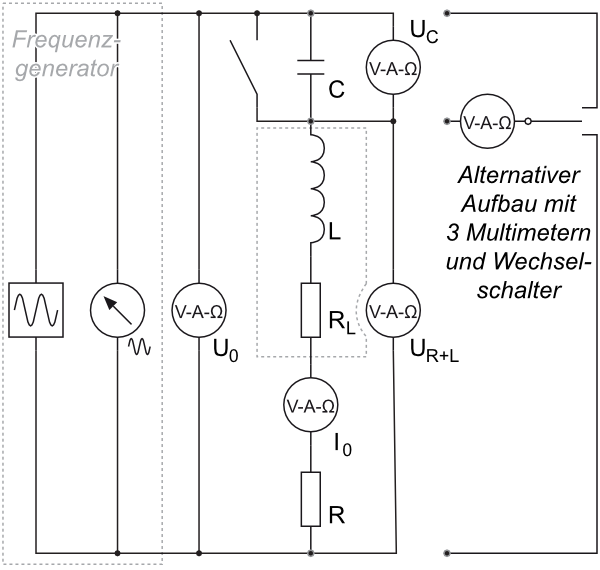
\includegraphics{reihe.png}
	\caption{Schaltskizze für den Serienkreis}
	\label{fig:schaltreihe}
\end{figure}
\begin{figure}[h!]
	\centering
	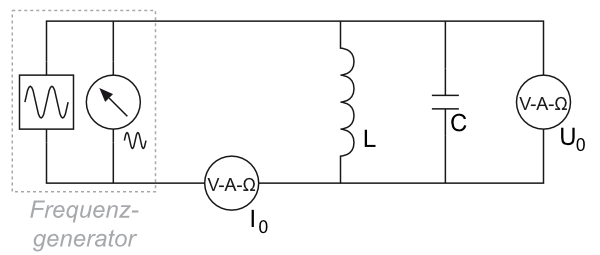
\includegraphics{para.png}
	\caption{Schaltskizze für den Parallelkreis}
	\label{fig:schaltpara}
\end{figure}

In den Abbildungen \ref{fig:schaltreihe} und \ref{fig:schaltpara} sind die Schaltskizzen der beiden Versuchsaufbauten zu sehen. Benötigt werden eine Wechselspannungsquelle mit variabler Frequenz, ein Kondensator, eine Luftspule, ein \person{Ohm}scher Widerstand, ein Schalter, ein Digitaloszilloskop und vier Multimeter. 
\subsection{Serienkreis ohne Kondensator}
\label{sec:serie1}
Für den ersten Versuchsteil werden die Bauteile gemäß Abbildungen \ref{fig:schaltreihe} in Reihe geschaltet. Der Schalter wird geöffnet, um den Kondensator zu überbrücken. Durch das Oszilloskop darf kein Strom fließen. Um die Phasenverschiebung zwischen Strom und Spannung zu messen, wird es deswegen sowohl direkt an die Spannungsquelle als auch parallel zum \person{Ohm}schen Widerstand geschaltet. Nun wird in einem Frequenzbereich von ca. 60 bis 80\;Hz für zehn verschiedene Frequenzen der Strom $I$ durch den \person{Ohm}schen Widerstand, die Gesamtspannung $U$ und die Phasenverschiebung  $\varphi$ zwischen Strom und Spannung gemessen. Die Spannung kann dabei an der Spannungsquelle eingestellt werden. Gemessen wird sie trotz der Anzeige der Spannungsquelle am Oszilloskop, da sie dort genauer ausgegeben wird. Die Phasenverschiebung ist ebenfalls am Oszilloskop abzulesen. Dafür muss sich dieses in dem Modus "`Messung"' befinden. Zu beachten ist, dass der Innenwiderstand des Amperemeters von dem eingestellten Messbereich abhängt. Um einer möglichen Verfälschung der Messwerte vorzubeugen, sollte deshalb für jeden Versuchsabschnitt ein einheitlicher Messbereich eingestellt werden. Die Widerstände der Voltmeter hingegen sind als unendlich angenommen.

\subsection{Serienkreis mit Kondensator}
Für diesen Versuchsteil wird der Schalter geöffnet, wodurch die Schaltung zu einem Serienschwingkreis wird. Wie in Sektion \ref{sec:serie1} wird für den gleichen Frequenzbereich die Gesamtspannung $U$, der Gesamtstrom $I$ und die Phasenverschiebung $\varphi$ gemessen. Hierbei ist darauf zu achten, die Resonanzstelle besonders genau abzutasten, um eine genaue Bestimmung der Resonanzfrequenz zu ermöglichen.

\subsection{Parallelkreis}
Nun wird der Parallelkreis ohne den \person{Ohm}schen Widerstand aus Abbildung \ref{fig:schaltpara} aufgebaut. Er besteht aus einer Spule  und einem parallelgeschalteten Kondensator. Der in der Spule integrierte Spulenwiderstand $R_L$ ist in Reihe zu dieser. Das Volt- und Amperemeter wird analog zu den Vorherigen Schaltungen angeschlossen. Erneut wird die Spannung $U$, der Strom $I$ und die Phasenverschiebung $\varphi$ notiert, wobei die Resonanzstelle besonders genau vermessen wird.
\subsection{Ausmessung der Bauteile}
Als letztes werden mit den Multimetern die elektrischen Bauteile vermessen. Hierzu gehören der Innenwiderstand des Amperemeters für alle verwendeten Messbereiche, der Widerstand des \person{Ohm}schen Widerstandes, der Widerstand der Spule, sowie die Kapazität des Kondensators. Ebenfalls zu notieren sind der Durchmesser und die Windungszahl der Luftspule.
\section{Auswertung}
\label{sec:auswertung}
\subsection{Bestimmung der Induktivität und des \person{Ohm}schen Widerstands beim Serienkreis ohne Kondensator}
Aus der Messreihe für den Serienkreis bei überbrücktem Kondensator (Sektion \ref{sec:serie1}) soll die Induktivität $L$ der Spule, sowie der gesamte \person{Ohm}sche Widerstand $R$, bestehend aus Spulenwiderstand $R_L$ und einzelnem \person{Ohm}schen Widerstand $R_\Omega$, bestimmt werden. Hierfür betrachtet man Gleichung \eqref{eq:zserie}. Da der Kondensator überbrückt ist, besteht der Imagiärteil  , woraus für den komplexen Widerstand $Z$ gilt:
\begin{align}
	Z(\omega)=R+i~\omega L.
	\label{eq:impedRL}
\end{align}
Berechnet man nun die Impedanz gemäß Gleichung \eqref{eq:impedanz} und quadriert, so erhält man
\begin{align}
	\left( \frac{U}{I} \right)^2=Z^2=\underbrace{R^2}_b+\omega^2 \underbrace{L^2}_m.
	\label{eq:gerade}
\end{align}
Man erwartet also einen linearen Zusammenhang zwischen dem Impedanzquadrat $Z^2$ und dem Quadrat der Kreisfrequenz $\omega^2$. Die Steigung $m$ entspricht dabei dem Quadrat der Induktivität $L^2$ und der Ordinatenabschnitt wird als Quadrat des \person{Ohm}schen Gesamtwiderstands $R^2$ identifiziert.
Für die Messfehler der Multimeter wurde der größtmögliche Fehler nach \cite[35]{prakti} verwendet, da die während des Versuchs angenommenen Fehler zu klein sind. Sie sind In Tabelle \ref{tab:messfehler} zu sehen.
\begin{table}
	\centering
	\begin{tabular}{l|l}
		\hline
		Messbereich&Fehler\\\hline
		alle Spannungen&$1\%$ v. Messwert + 3 Digits\\
		alle Ströme&$1.5\%$ v Messwert + 3 Digits\\\hline
	\end{tabular}
	\caption{Messfehler der Multimeter}
	\label{tab:messfehler}
\end{table}
Der Fehler der Frequenz wurde einheitlich auf $\sigma_f=1$ gesetzt, da der auf dem Oszilloskop ausgegebene Wert innerhalb dieses Bereichs schwankte. Das Kreisfrequenzquadrat berechnet sich nach $\omega^2=\left( 2\pi f \right)^2$. Mit der \person{Gauss}schen Fehlerfortpflanzung ergibt sich ein Fehler von 
\begin{align}
	\sigma_{\omega^2}=8  \pi^{2}  f\cdot \sigma_{f}.
	\label{eq:sigmaomega}
\end{align}
 Der Fehler der gesamten Impedanz berechnet sich nach
\begin{align}
	\sigma_{Z_0^2}=\frac{2}{I^{3}} \cdot U \cdot \sqrt{I^{2} \cdot \sigma_{U}^{2} + U^{2} \cdot \sigma_{I}^{2}}.
	\label{eq:sigmaz0}
\end{align}
\begin{figure}[h!]
	\centering
	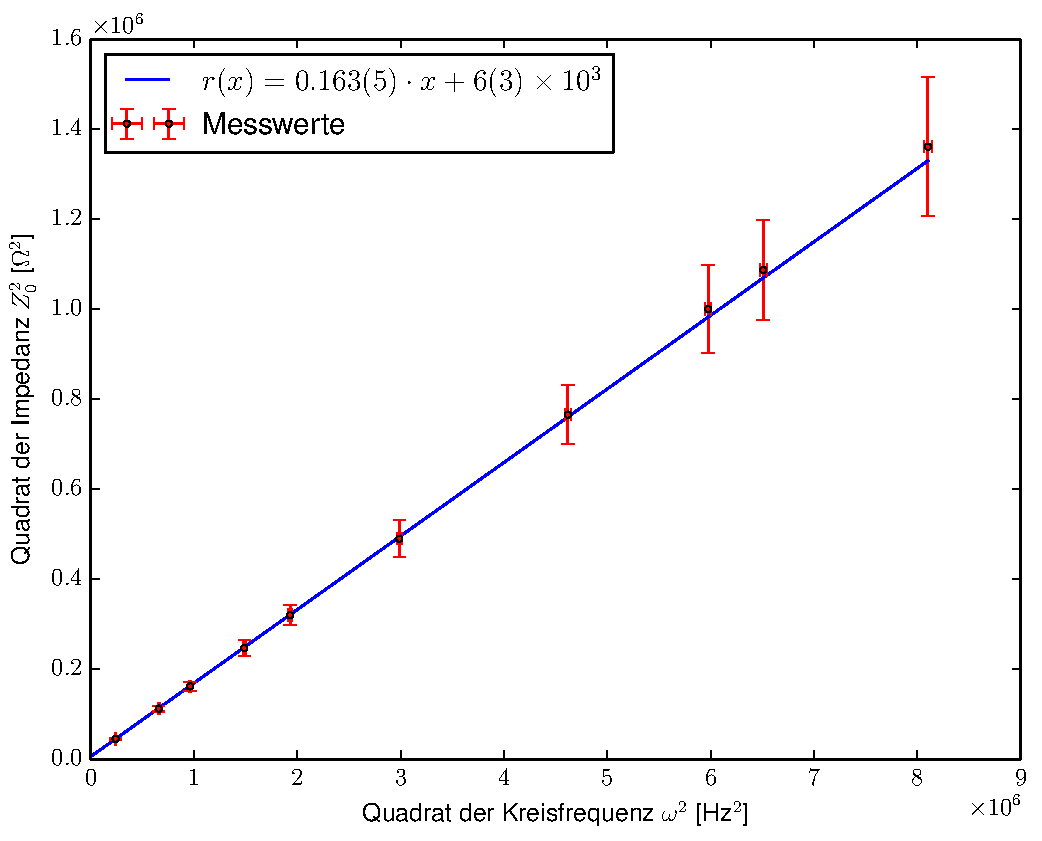
\includegraphics[width=\textwidth]{plot1.pdf}
	\caption{Auswertung des Serienkreises ohne Kondensator. Das Quadrat der Impedanz wird über dem Quadrat der Kreisfrequenz aufgetragen. Es ergibt sich wie erwartet ein linearer Zusammenhang. In rot sind die Messwerte samt Fehler, in blau ist die Regressionsgerade aufgetragen.}
	\label{fig:plot1}
\end{figure}

Die Auftragung des Impedanzquadrates über dem Kreisfrequenzquadrat ist in Abbildung \ref{fig:plot1} zu sehen. Anschließend wird eine lineare Regression durchgeführt. Die Regressionsgerade ist ebenfalls in Abbildung \ref{fig:plot1} eingezeichnet. Man erhält als Parameter:
\begin{align}
	m&=L^2=(0.163\pm0.005)~\mrm{H}^2\\
	b&=R^2=(6\pm3)\times 10^3~\mrm{\Omega}^2
	\label{eq:plot1}
\end{align}
Nach \person{Gauss} ergibt sich für die Fehler von Induktivität $L$ und Widerstand $R$:
\begin{align}
	\sigma_L=\frac{1}{2\sqrt{m}}\cdot\sigma_m,\qquad\sigma_R=\frac{1}{2\sqrt{m}}\cdot\sigma_b.
	\label{eq:sigma1}
\end{align}
Es ergeben sich als Resultate:
\begin{align}
	L=(0.404\pm0.007)~\mrm{H}\\
	R=(76\pm18)~\mrm{\Omega}.
	\label{eq:result1}
\end{align}
\subsection{Bestimmung der Resonanzfrequenz und des \person{Ohm}schen Widerstands beim Serienresonanzkreis}
\begin{figure}[h!]
	\centering
	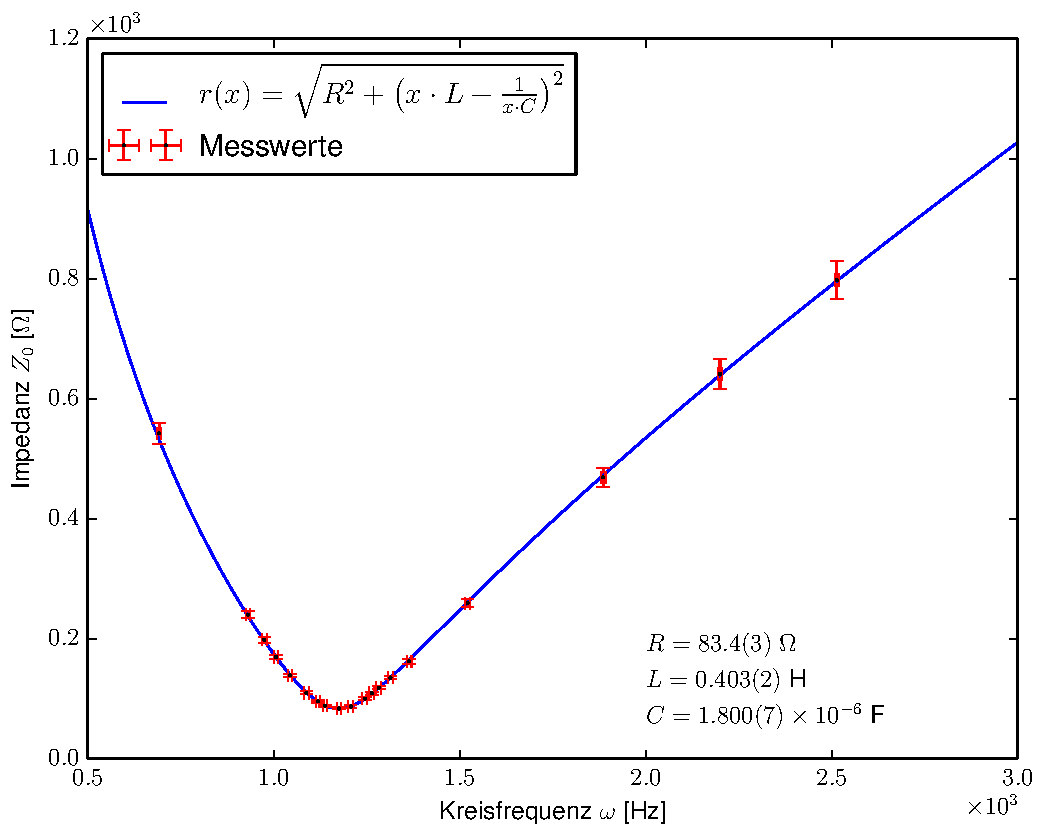
\includegraphics[width=\textwidth]{plot2.pdf}
	\caption{blablabla}
	\label{fig:plot2}
\end{figure}
\begin{figure}[h!]
	\centering
	\input{zeiger2.pdf_tex}
	\caption{BLAH}
	\label{fig:zeiger2}
\end{figure}


\section{Diskussion}
\label{sec:diskussion}

\newpage
%\nocite{*} %sorgt dafuer, dass alles ausgegeben wird
\printbibliography[heading=bibintoc]
\end{document}
